%%%%%%%%%%%%%%%%%%%%%%%%%%%%%%%%%%%%%%%%%
% Short Sectioned Assignment
% LaTeX Template
% Version 1.0 (5/5/12)
%
% This template has been downloaded from:
% http://www.LaTeXTemplates.com
%
% Original author:
% Frits Wenneker (http://www.howtotex.com)
%
% License:
% CC BY-NC-SA 3.0 (http://creativecommons.org/licenses/by-nc-sa/3.0/)
%
%%%%%%%%%%%%%%%%%%%%%%%%%%%%%%%%%%%%%%%%%

%----------------------------------------------------------------------------------------
%	PACKAGES AND OTHER DOCUMENT CONFIGURATIONS
%----------------------------------------------------------------------------------------

\documentclass[letterpaper]{scrartcl} % A4 paper and 11pt font size

\usepackage[T1]{fontenc} % Use 8-bit encoding that has 256 glyphs
\usepackage{fourier} % Use the Adobe Utopia font for the document - comment this line to return to the LaTeX default
\usepackage[english]{babel} % English language/hyphenation
\usepackage{amsmath,amsfonts,amsthm} % Math packages

\usepackage{lipsum} % Used for inserting dummy 'Lorem ipsum' text into the template

\usepackage{sectsty} % Allows customizing section commands
\allsectionsfont{\normalfont\scshape}
%\allsectionsfont{\centering \normalfont\scshape} % Make all sections centered, the default font and small caps

\usepackage{graphicx}

\usepackage{hyperref}
\hypersetup{
    colorlinks=true,
    linkcolor=blue,
    filecolor=blue,
    urlcolor=blue,
    citecolor=blue,
}

\usepackage{listings}
\usepackage{color}

\definecolor{dkgreen}{rgb}{0,0.6,0}
\definecolor{gray}{rgb}{0.5,0.5,0.5}
\definecolor{mauve}{rgb}{0.58,0,0.82}

\lstset{frame=tb,
  language=Java,
  aboveskip=3mm,
  belowskip=3mm,
  showstringspaces=false,
  columns=flexible,
  basicstyle={\small\ttfamily},
  numbers=none,
  numberstyle=\tiny\color{gray},
  keywordstyle=\color{blue},
  commentstyle=\color{dkgreen},
  stringstyle=\color{mauve},
  breaklines=true,
  breakatwhitespace=true,
  tabsize=3
}

\usepackage{fancyhdr} % Custom headers and footers
\pagestyle{fancyplain} % Makes all pages in the document conform to the custom headers and footers
\fancyhead{} % No page header - if you want one, create it in the same way as the footers below
\fancyfoot[L]{} % Empty left footer
\fancyfoot[C]{} % Empty center footer
\fancyfoot[R]{\thepage} % Page numbering for right footer
\renewcommand{\headrulewidth}{0pt} % Remove header underlines
\renewcommand{\footrulewidth}{0pt} % Remove footer underlines
\setlength{\headheight}{13.6pt} % Customize the height of the header

\numberwithin{equation}{section} % Number equations within sections (i.e. 1.1, 1.2, 2.1, 2.2 instead of 1, 2, 3, 4)
\numberwithin{figure}{section} % Number figures within sections (i.e. 1.1, 1.2, 2.1, 2.2 instead of 1, 2, 3, 4)
\numberwithin{table}{section} % Number tables within sections (i.e. 1.1, 1.2, 2.1, 2.2 instead of 1, 2, 3, 4)

\setlength\parindent{0pt} % Removes all indentation from paragraphs - comment this line for an assignment with lots of text

%----------------------------------------------------------------------------------------
%	TITLE SECTION
%----------------------------------------------------------------------------------------

\newcommand{\horrule}[1]{\rule{\linewidth}{#1}} % Create horizontal rule command with 1 argument of height

\title{
\normalfont \normalsize
\textsc{Fundamentals of Computer Networks, Final Project Report} \\ [25pt] % Your university, school and/or department name(s)
\horrule{0.5pt} \\[0.4cm] % Thin top horizontal rule
\huge Evaluating the Effectiveness of JavaScript Crypto Miner Blocker Browser Extensions \\ % The assignment title
\horrule{2pt} \\[0.5cm] % Thick bottom horizontal rule
}

\author{Babak Amin Azad (111740448), Avinash Kumar (111471353)} % Your name

\date{\normalsize\today} % Today's date or a custom date

\begin{document}

\maketitle % Print the title

%----------------------------------------------------------------------------------------
%	PROBLEM 1
%----------------------------------------------------------------------------------------

\section{Introduction}
\paragraph{}
JavaScript crypto miners have been around for quite a while. Monero (XMR), the crypto currency mined by these scripts was released in April 2014. As shown in Figure~\ref{fig:bitcoin-increase-price}, the increase in price of Bitcoin was coupled with increase in price of Ethereum and Monero. This jump led to these in browser miners being over emphasized in the media.

\begin{figure}[t]
\centering
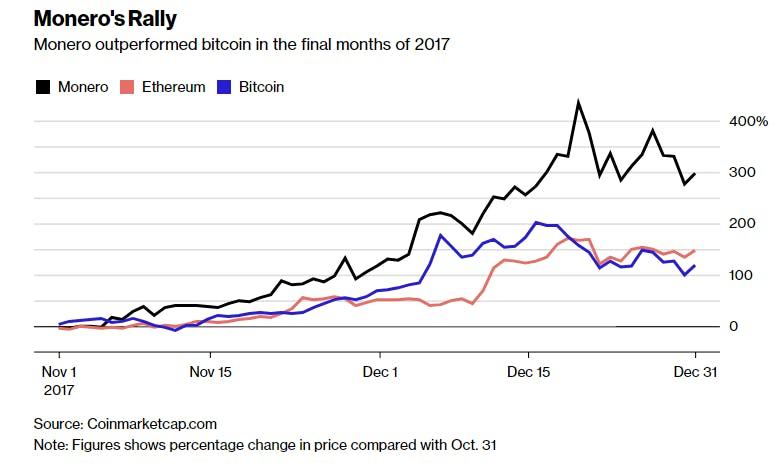
\includegraphics[width=0.8\columnwidth]{figures/bitcoin-increase-price.jpeg}
\caption{Price comparison between Bitcoin, Ethereum and Monero }
\label{fig:bitcoin-increase-price}
\end{figure}

\section{Analysis of JavaScript crypto miners}
\paragraph{}
With the rise of JavaScript crypto miners, website administrators started including miner scripts in their websites. The more the user stays on the website, the more Monero mined. ``Coinhive review: Embeddable JavaScript Crypto Miner - 3 days in''~\cite{ref:medium-coinhive} shows that using JavaScript crypto miners in place of advertisements provides a marginally smaller revenue. The takeaway is that miners can't replace ads, but using both of them or using miners specifically on websites where users spend more time like video sharing or gaming websites can increase the income.

\subsection{Replacing annoying advertisements with annoying miners}
\paragraph{}
Many of us use ad blockers to prevent advertisements being shown on websites when we are surfing the web. Use of these blockers brings up many arguments and ethical concerns, since advertisements are usually the source of income for websites, by blocking them the income for these websites is being limited. On the other hand we see Malwaretisement campaigns abusing ad networks to distribute their malware and compromise users' machines. As websites started including miners in their pages, users started using miner blocker extensions to stop the miners from running. In this study we analysed top miner blocker extensions for Firefox and Google Chrome and report on their effectiveness. List of analysed extensions is available in the Table~\ref{tab:analysed-extensions}):

\begin{table}[]
\centering
\caption{List of analysed browser extensions}
\label{tab:analysed-extensions}
\begin{tabular}{lc}
\hline
\multicolumn{1}{|l|}{\textbf{Firefox}}                        & \multicolumn{1}{|l|}{\textbf{Chrome}} \\ \hline
\multicolumn{1}{|l|}{\href{https://addons.mozilla.org/en-US/firefox/addon/no-coin/}{No Coin} (84,524 Users)}         & \multicolumn{1}{|l|}{\href{https://chrome.google.com/webstore/detail/no-coin-block-miners-on-t/gojamcfopckidlocpkbelmpjcgmbgjcl?hl=en}{No Coin} (570,185 Users)}    \\ \hline
\multicolumn{1}{|l|}{\href{https://addons.mozilla.org/en-US/firefox/addon/nominer-block-coin-miners/}{No Miner} (28,413 Users)}        & \multicolumn{1}{|l|}{\href{https://chrome.google.com/webstore/detail/minerblock/emikbbbebcdfohonlaifafnoanocnebl?hl=en}{Miner Block} (157,807 Users)} \\ \hline
\multicolumn{1}{|l|}{\href{https://addons.mozilla.org/en-US/firefox/addon/minerblock-origin/}{Miner Block} (15,557 Users)}     & \multicolumn{1}{|l|}{\href{https://chrome.google.com/webstore/detail/crypto-miner-blocker/fekkecoifalagdiibmfnmjfmgmpblogb?hl=en}{CryptoMiner Blocker} (5,811 Users)}     \\ \hline
\multicolumn{1}{|l|}{\href{https://addons.mozilla.org/en-US/firefox/addon/miningblocker/}{Mining Blocker} (12,187 Users)}  & \multicolumn{1}{|l|}{} \\ \hline
\end{tabular}
\end{table}

\paragraph{}
``No Coin'' extension on Google Chrome, has more than half a million installation from Chrome store. In the next step we analyse the source code of these extensions. Turns out the same method of blocking is used in nearly all of them. A set of regex statements that match URLs that the main javascript for known miners are hosted on, one example of this would be:

\begin{lstlisting}
https://coinhive.com/lib/coinhive.min.js
\end{lstlisting}
and the regex matching this script for different miner blocker extensions is:
\begin{lstlisting}
*://*.coinhive.com/*
*://*/*coinhive*.js*
*://coinhive.com/lib*
*://*.coinhive.com/lib/*
*://*/*coinhive.min.js*
\end{lstlisting}

\paragraph{}
Existing method in extensions to block miners is by detecting and blocking the main JavaScript library that has to be included in web pages. As you already noticed, by self hosting these scripts one can trivially bypass these blockers. Now let's use PublicWWW to find out how many miners on the web actually include these JavaScript libraries from the provided URLs.

\begin{figure}[t]
\centering
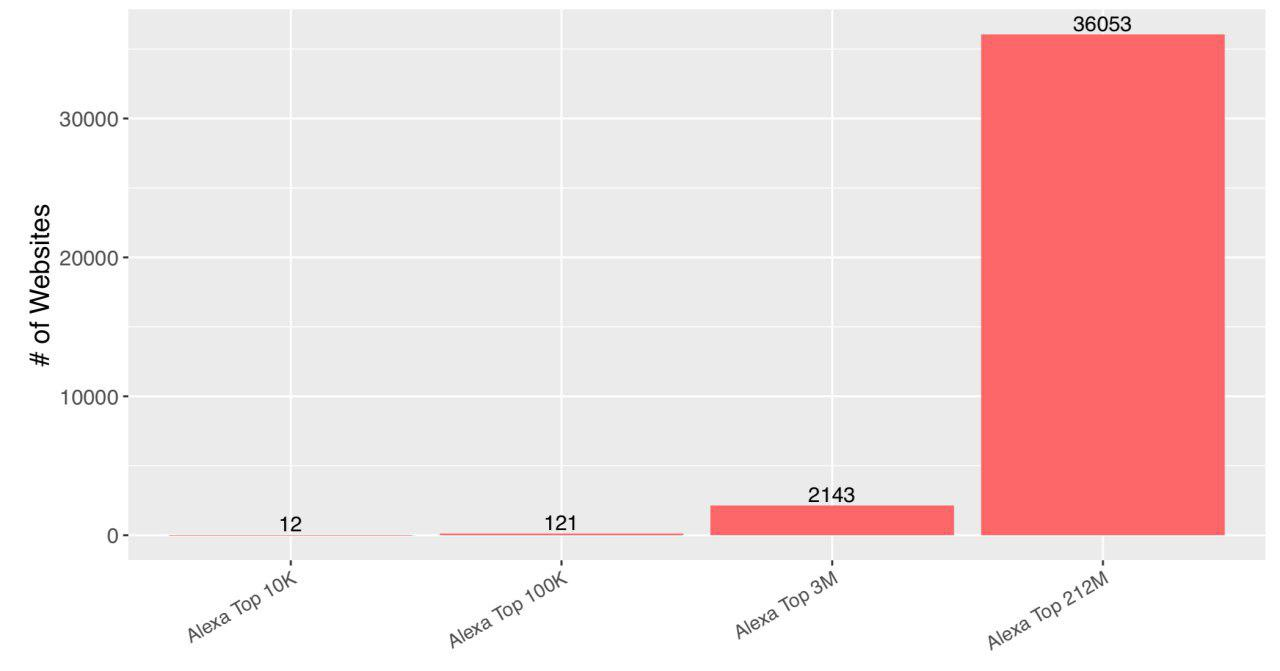
\includegraphics[width=0.8\columnwidth]{figures/miners-on-top-alexa.jpg}
\caption{Distribution of websites using miner scripts}
\label{fig:miners-on-top-alexa}
\end{figure}

\paragraph{}
Based on signatures derived from browser extensions, as depicted in Figure~\ref{fig:miners-on-top-alexa}, we found only 12 websites in top 10k Alexa websites, this number grows linearly and reaches 36053 for Top 212M Alexa websites. This would either mean that top Alexa websites do not use miners, or it could mean that they actively try to hide their miners which makes miner blocker extensions useless.

\paragraph{}
Now let's look at the websites which use miners from another view, for this part of the report, \href{https://fortiguard.com/webfilter}{https://fortiguard.com/webfilter}, is used to categorize the URLs, since most of these samples are not well known websites, the category won't be present for most of them, but out of those which we could find a category for, this is the top ones:

\begin{enumerate}
\item Malicious Websites
\item Business
\item Information Technology
\item Pornography
\item Personal Websites and Blogs
\end{enumerate}

Next, we analyze which miners are more popular in Figure~\ref{fig:miner-providers}

\begin{figure}[t]
\centering
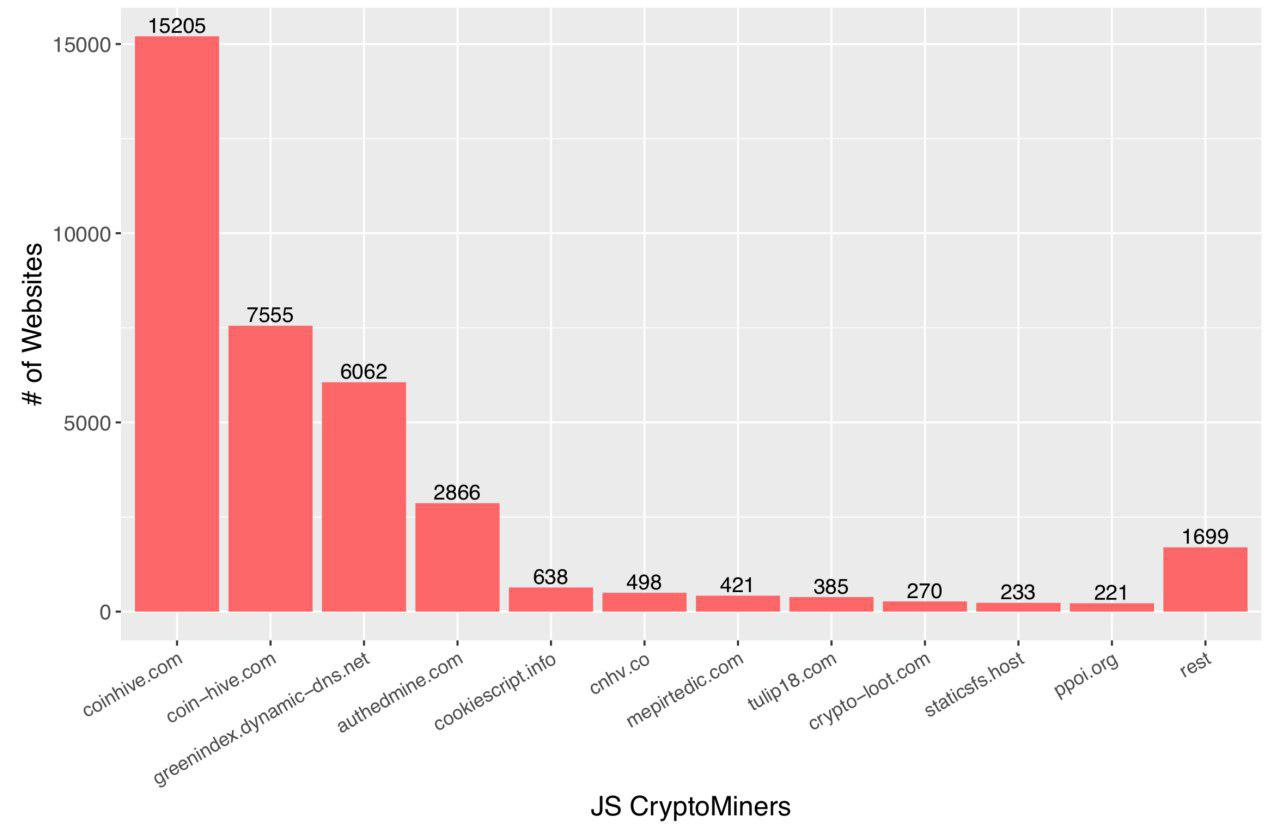
\includegraphics[width=0.8\columnwidth]{figures/miner-providers.jpg}
\caption{Miner script providers and their number of clients on Alexa top 212M}
\label{fig:miner-providers}
\end{figure}

\paragraph{}
Figure~\ref{fig:miner-providers} has a couple of interesting findings, first, coinhive and its other domains (coinhive.com, coin-hive.com, cnhv.co) together make up the most popular miners used by websites on the web. Next we have authedmine.com, which also belongs to coinhive, but this service explicitly asks the user for permission to mine on his computer, this is due to the fact that mining without users' concent was deemed as a malicious act and browser extensions started blocking them. To prevent it, coinhive proposed authedmine as a fully ``ethical'' counterpart of their original service.

\paragraph{}
On this list we also see crypto-loot, which is a new player in this game, they provide 80\% of the mining income to website administrators compared to 70\% revenue share for admins using coinhive.
``rest'' category is the sum of samples with presence on less than 200 websites on Alexa top 212M websites.

\paragraph{}
On this list, we see greenindex.dynamic-dns.net which looks to be a non-miner website. Our first guess was that someone hosted a miner script on their website. After doing some research, we get to their website which looks benign. They host \href{https://greenindex.dynamic-dns.net/jqueryeasyui.js}{https://greenindex.dynamic-dns.net/jqueryeasyui.js} which is a version of deepMiner, which is a self hosted cryptominer. Various blogs point out that this miner is used in a malicious way, as in being injected into compromised websites. deepMiner has a feature to limit the amount of its CPU utilizations, and in some of the compromised websites with this specific miner URL in them, this value was set to 0.5, preventing full cpu utilization by the script as referenced by ``The Growing Trend of Coin Miner JavaScript Infection''~\cite{ref:fortinet-minerinfection}.

\paragraph{}
Another benign looking domain is cookiescript.info. They advertise themselves as:

\textbf{The most popular free solution to US and European Cookie Laws:}

``\textit{European and American laws require that digital publishers give visitors to their sites and apps information about their use of cookies and other forms of local storage. These laws also require that consent be obtained. A breach of these regulations can result in a fine of up to \$500,000.}''

As it turns out, these guys have been abusing their script that users would include in their website to mine cryptocurrencies. The two following URLs are examples of mining scripts present on this domain:

\begin{lstlisting}
http://cdn.cookiescript.info/libs/cookieconsent.5.min.js
https://cdn.cookiescript.info/libs/cookiescript.min.js
\end{lstlisting}
\paragraph{}
The author of ``CookieScript.info mining Monero on your website?! It's true''~\cite{ref:cookiescript}, claims that cookiescript moderators have been contacted and no response was received as of the writing.

\subsection{Analyzing the miner scripts}
\paragraph{}
We extracted the list of URLs that host JavaScript miner scripts. They can be used in a future research but for now, we tested their reachability. Following are some samples of URLs with invalid SSL certificates, Figure~\ref{fig:miner-invalid-certificate} is one example of such cases:
\begin{lstlisting}
https://staticsfs.host/js/EQHAwxADAgAUxAGS
https://gtg02.bestsecurepractice.com/meri.js
\end{lstlisting}

\begin{figure}[t]
\centering
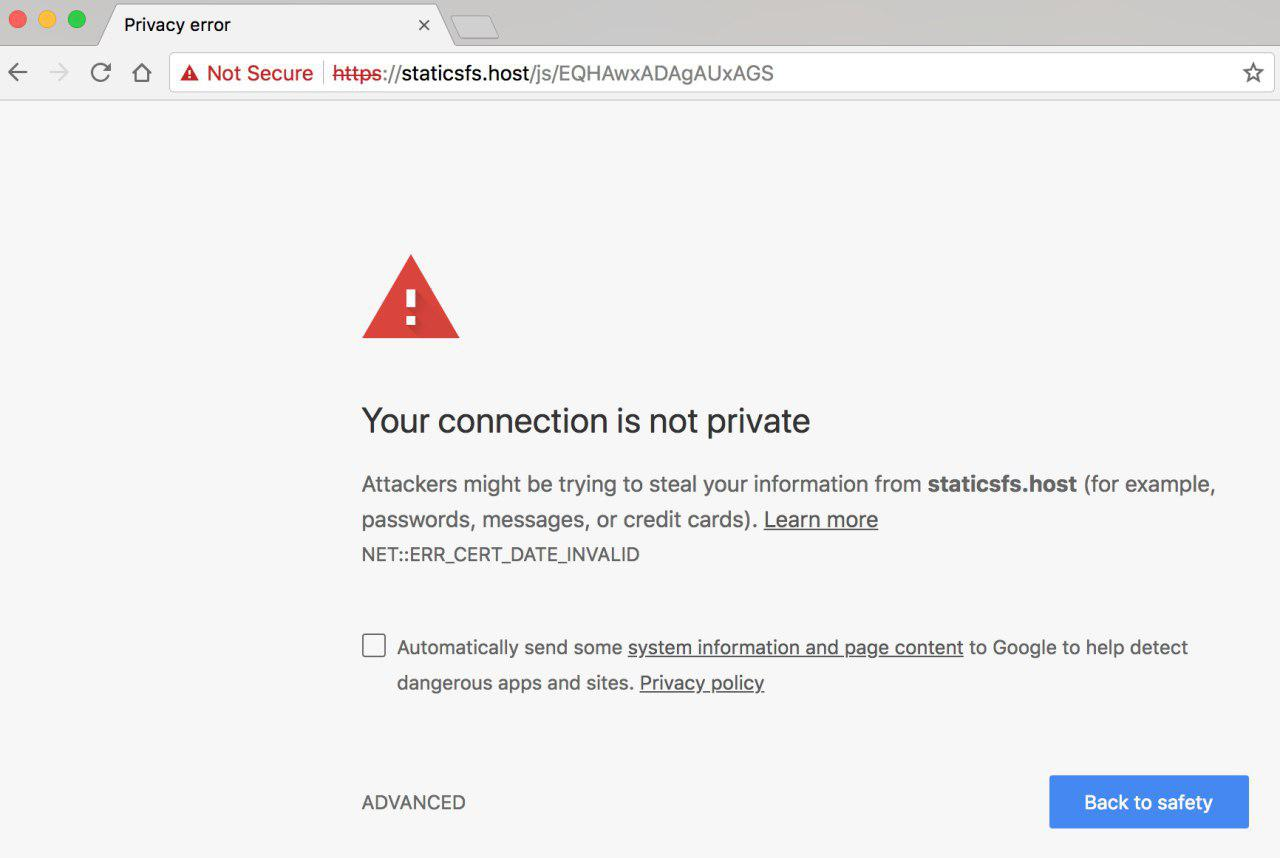
\includegraphics[width=0.8\columnwidth]{figures/miner-invalid-certificate.jpg}
\caption{Example of miner script being hosted with invalid certificate}
\label{fig:miner-invalid-certificate}
\end{figure}

\paragraph{}
These samples were using let's encrypt, they might have forgotten to setup auto renew script to renew certificates, but the outcome of this is that websites that include these JavaScript files won't be able to mine because browsers will not fetch scripts hosted in websites with invalid SSL certificates. This was also reported recently on twitter by \textit{@bad\_packets}, a malicious actor managed to break into a government website, but due to invalid SSL certificate of the website hosting his miner, he failed to mine crypto currency.

\subsection{Malicious Miners}
\paragraph{}
Now the question arises, are these the true number of websites using crypto miners? Or are there many other self hosted and malicious miners that obfuscate themselves and their URLs to stay hidden? To answer this question we can refer to ``Unauthorized Coin Mining in the Browser''~\cite{ref:pan-mining}, where the author from Palo Alto Networks uses their own dataset of passive DNS and logs from their devices, shows that they observe roughly the same number of malicious infected websites by miner campaigns as we observed by using signatures used in miner blocked browser extensions.

\section{Technical \& implementation details}
\paragraph{\textbf{Browser extensions as ground truth source of data}}
We reverse engineered top crypto miner blocker extensions and got the list of the miners signatures.
This list was then refined to remove the duplicates and non-exiting miners. Analyzed extensions are available at

 \href{https://github.com/silverfoxy/JSCryptoMinerStudy/tree/master/JSCryptoBlockerAddons}{https://github.com/silverfoxy/JSCryptoMinerStudy/tree/master/JSCryptoBlockerAddons}.

\subsection{Choice of datasource}
\paragraph{\textbf{Common Crawl}}
We started with the idea of crawling top alexa sites (1M) on our won to fetch the page source and run
our analysis on top of them. We decided to use Common Crawl datasource as our input http://commoncrawl.org/the-data/, which could provide us with
periodic crawls and stored data of web pages of our need. We downloaded top 10k Alexa pages from there
and ran our analysis code to look for the miners. Our approach was to find all possible exitence of miner
scripts, hence instead fo looking for just the mining script provider, we looked for all the possible regexes
which could be a possible miner. We had the task of matching about 1,000 regexes with 10,000 pages. Using a
single computer to run this task turned out to be very time consuming as one regex unfolds to many
strings and even Python's standard regex libraries took too much time to yield results.

\paragraph{}
We modified our code to just look for the miner URLs, in place of all the regexes to bring
down the run time. With Alexa top 10,000 pages, we did not find enough results to draw out some relevant conclusions. As we later supported this observation by PublicWWW, only 12 miners could be found on this subset of websites using signatures from browser extensions.

\paragraph{\textbf{PublicWWW}}
We decided to go ahead with larger number of sites and we came across

https://publicwww.com/,
a source code search engine. Apart from listing results and providing facility to download pages,
it also exposes some APIs to fetch the result in csv format. We developed code to work with those APIs to get
the data. And top of it we developed additional code to fetch relevant details for our analysis and plotting.

\subsection{implementation details}
\paragraph{\textbf{The code}} is hosted on github (\href{https://github.com/silverfoxy/JSCryptoMinerStudy}{https://github.com/silverfoxy/JSCryptoMinerStudy}). The repository has additional data and scripts which we used in former stages of the project, due to the nature of our study which included lots of data gathering, cleaning and analysis, we developed Python and Bash scripts to help us through different stages. The main code lies
in the directory \textit{pubwww}.

\subsubsection{Usage}
\paragraph{}
\textbf{python crawlpubwww.py}:
fetches following data:
\begin{itemize}
\item \textbf{pages} : for each miner, list of pages contaning that miner and total number of such pages, displayed
as summary src of pubwww displaying the results summary of miner search, count + list
\item \textbf{csvs} : csvs(url, rank, script\_src) of the list of sites containing the particular miner
\item \textbf{script} : csvs(url, rank, script\_src\_found) of miners using JS mining
\item \textbf{wss} : csvs(url, rank, wss\_src\_found) of miners using web sockets for mining
\end{itemize}

\paragraph{}
\textbf{python miner\_counter.py}:
crawls through the fetched pages and reports the summary of a particula miner in total results

\subsubsection{Crawled Data}
All the crawled data lies in the following directories:
\begin{itemize}
\item \textbf{pubwww/data}
\item \textbf{pubwww/pages}
\item \textbf{pubwww/script}
\item \textbf{pubwww/wss}
\item \textbf{pubwww/csvs}
\end{itemize}

\section{Conclusion}
\paragraph{}
To study the effectiveness of available miner blocker browser extensions, we extracted the signatures used by these extensions, all observed extensions try to statically find URLs that are known to host JavaScript libraries used by these miners. Their database of signatures contain a high amount of false positive and dead links, as we were able to reduce aggregated list of 1000 signatures to ~100 valid and live URLs actively hosting miner scripts.

\paragraph{}
We also show that at best, these extensions are able to detect half of known miners and website moderators can trivially bypass these extensions by self hosting and obfuscating their mining scripts. Hence, a more concrete and dynamic approach is required to detect and block JavaScript crypto miners on the web.

\section{Future work}
\paragraph{}
Our framework of data gathering can be run periodically to gather and compare the results
to understand the usage pattern of JavaScript based crypto miners on
the websites, by having access to enough computation resource, we can run our analysis over monthly crawls of Common Crawl dataset
and correlate between zero-day vulnerabilities on famous websites e.g., Wordpress, Drupal, etc. and their effect on rise of number of websites
that have miner scripts in them, we can also add the feature to track API keys for miners and track malicious campaigns abusing bugs to inject
their own miner scripts into target websites and earn money from websites' visitors. Based on
the primary information from the current study, we may crawl the specific sites where we saw the
presence of miners, and derive some conclusion about, how effectively browsers work with or without
blocking them. The fact that current approach used by miner blocker extensions isn't effective also points
at a new area of research and future work, trying to detect miners
while being URL and file agnostic, maybe behavioral analysis can be applied to scripts and find anomalies and
malicious high CPU usage and put a limit on the amount of resource JavaScript files can use.

\bibliographystyle{unsrt}
\bibliography{references}
\end{document}
